
\subsection{Container Networking with \wnet}

\wnet\ was choses because, to this date, it is the only solution that supports both, multicast and encryption. Competing tools are flannel and dockernet.

Features: Own DNS Server to allow for looking up containers by its hostname. Dynamic Topologies: New containers can be easily included into the existing network. Self-governing: Weave Net peers continually exchange topology information, and monitor and (re)establish network connections to other peers (IMPORTANT for dynamic environment)

Advantages: No key-value store required

\paragraph{Encryption.} 
IPsec-based. Each packet is encapsulated in the ESP. Encryption is built using the Linux Crypto API

For sleeve mode:
Curve25519, XSalsa20 and Poly1305
Similar to TLS, but unlike TLS, Weave encryption supports UDP.


All traffic flows through three ports: one of type TCP and two of type UDP.

\begin{figure}[htpb]
  \centering
  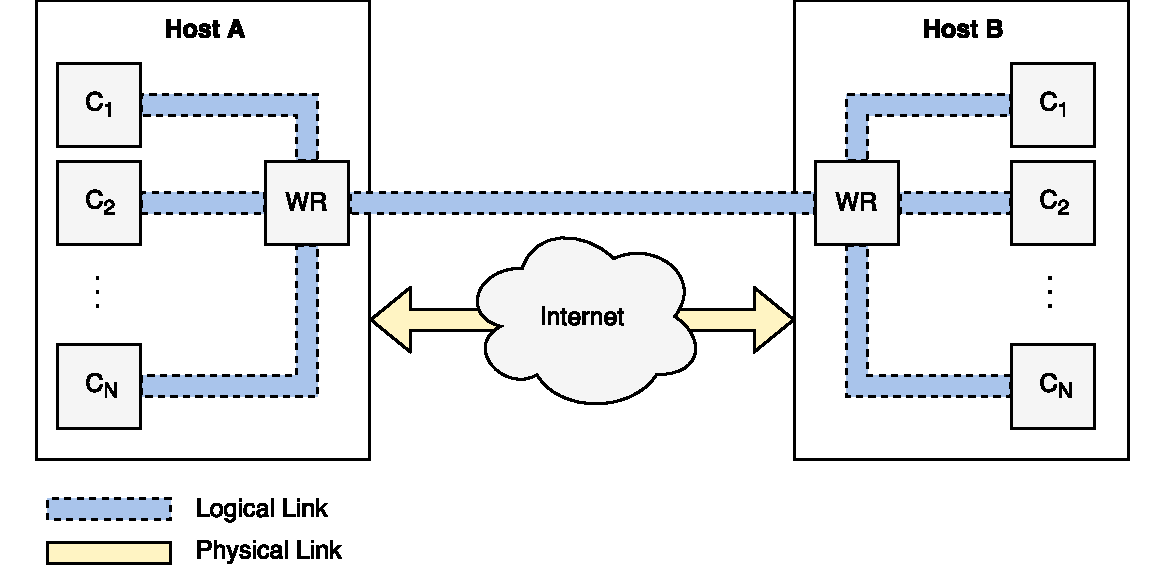
\includegraphics[width=\textwidth]{figures/sdn.pdf}
  \caption[SDN]{Connecting containers using \wnet }\label{fig:weave}
\end{figure}

Drawbacks: \wnet\ does not support IPv6 which is to the detriment of IoT networks, which benefit from the vast number of addresses of IPv6. However, in the vehicle use case, it is rather unlikely that every ECU has its own IP address. Rather, there is one gateway connected to a 5G module and all traffic is routed through that gateway. Because of this, the address scarcity issue only peripherally applies to the intended use case.